\apendice{Especificación de Requisitos}

\section{Introducción}
En este apartado se detallarán todos los requisitos, tanto funcionales como no funcionales, que tiene que cumplir el producto para abarcar los objetivos iniciales propuestos, es decir, se comprobará si las funcionalidades del producto cumplen con lo esperado.
\section{Objetivos generales}
Los objetivos que se desean alcanzar con el desarrollo del proyecto son los siguientes:
\begin{itemize}
\tightlist
	\item Desarrollar un videojuego de género \textit{shooter}, en concreto del estilo \textit{battle royale}, para ordenador como plataforma de juego, compatible con Windows y Linux y pensado para controlarse con teclado y ratón. Este objetivo puede subdividirse a su vez en objetivos más concretos:
    	\begin{itemize}
    	\tightlist
    	\item Desarrollar una buena \textbf{jugabilidad} y mecánicas interesantes para que el producto resulte entretenido y divertido para los usuarios.
    	\item Hacer que el producto sea \textbf{accesible} para un gran espectro de usuarios, es decir, que aprendan las mecánicas y acciones que ofrece el videojuego de forma intuitiva y con una curva de aprendizaje sencilla y no frustrante.
    	\item Crear de manera \textbf{autónom}a la mayoría de componentes del videojuego, incluyendo scripts, modelos, texturas, efectos, elementos de interfaces y sonidos.
    	\item Hacer que el videojuego sea \textbf{óptimo} en términos de rendimiento.
    	\item Utilizar \textbf{patrones, algoritmos y estructuras} de programación convenientes en cada caso.
    	\item Hacer que el proyecto sea fácilmente \textbf{extensible} para incluir mecánicas, objetos, mejoras o modificaciones de manera sencilla e intuitiva.
    	\end{itemize}
	\item Aprender el funcionamiento y las características fundamentales de Unity, así como del lenguaje de programación que utiliza (C\#)
	\item Aplicar la metodología \textit{Kanban} durante el desarrollo del producto para la gestión de las tareas.
	\item Integrar Git y Github como sistema de control de versiones.
	\item Asentar las bases de conocimiento personal para poder realizar otros proyectos similares en el futuro o continuar el desarrollo y mejora del mismo.
\end{itemize}
\section{Catalogo de requisitos}
En este apartado se detallarán cada uno de los requisitos del producto. Estos se pueden dividir, dependiendo de su naturaleza, en dos categorías: \textbf{funcionales} y \textbf{no funcionales}.

\subsection{Requisitos funcionales}
Son los servicios y funciones que el sistema debe ofrecer ante la interacción de los usuarios con él.
\begin{itemize}
    \item \textbf{RF-1 Iniciar sesión}: El jugador debe poder ser identificado de manera única e inequívoca para diferenciarse de los demás jugadores existentes en la aplicación y acceder a su cuenta.
    \begin{itemize}
        \item \textbf{RF-1.1 Registro}: El usuario debe poder registrarse en el juego introduciendo sus datos como nombre de usuario, correo y contraseña para crear una cuenta.
    \end{itemize}
    \item \textbf{RF-2 Gestión del menú principal}: Debe haber un menú central desde el que se pueda navegar a las distintas secciones de la aplicación.
    \begin{itemize}
        \item \textbf{RF-2.1 Mostrar datos del jugador}: El jugador debe poder ver su nombre de usuario y su experiencia total en el menú principal.
        \item \textbf{RF-2.2 Gestión del Menú de opciones}: El jugador debe poder acceder a un menú de opciones generales del juego y así poder modificar algunos aspectos generales del juego como la resolución, la calidad gráfica o el volumen del sonido.
        \item \textbf{Ver Clasificación}: El jugador debe poder ver quiénes son los jugadores que más experiencia han acumulado en el juego en forma de lista, actualizándose esta cada vez que se consulte.
        \item \textbf{RF-2.4 Cerrar sesión}: El jugador debe poder cerrar su sesión de usuario.
        \item \textbf{RF-2.5 Salir del juego}: El jugador debe poder salir de la aplicación cuando lo desee.
    \end{itemize}
    \item \textbf{RF-3 Jugar}: El sistema debe permitir iniciar y desarrollar una partida.
    \begin{itemize}
        \item \textbf{RF-3.1 Generación de mapa}: El juego debe ser capaz de generar un mapa al inicio de la partida de forma procedural y única en cada partida.
        \item \textbf{RF-3.2 Mover al jugador}: El jugador debe poder moverse en cualquier dirección sobre el terreno, según el input que se reciba del usuario.
        \begin{itemize}
            \item \textbf {RF-3.2.1 Deslizarse}: El jugador debe poder deslizarse por el terreno si así lo desea y si el terreno es lo suficientemente inclinado
            \item \textbf{RF-3.2.2 Correr por la pared}: el jugador debe poder correr por las paredes y saltar desde ellas a otras paredes para moverse de manera más dinámica y que pueda alcanzar lugares altos de difícil acceso.
        \end{itemize}
        \item \textbf{RF-3.3 Mirar alrededor}: El jugador debe poder mirar a su alrededor, dirigiendo la mirada donde el usuario desee.
        \item \textbf{RF-3.4 Saltar}: El jugador debe poder saltar, elevándose en el aire.
        \begin{itemize}
            \item \textbf{RF-3.4.1 Usar trampolín}: El jugador debe poder saltar sobre una plataforma de rebote que le impulse varios metros en el aire para llegar a lugares altos o huir de algún sitio.
        \end{itemize}
        \item \textbf{RF3.5 Abrir caja de suministros}: El jugador debe poder abrir las cajas de suministros que encuentre.
        \item \textbf{RF3.6 Equipar armamento}: El jugador debe poder equipar y añadir a su inventario objetos de armamento que encuentre en cajas o en el suelo, como armas o granadas, hasta poder llenarlo por completo.
        \item \textbf{RF-3.7 Desequipar armamento}: El jugador debe poder desequipar el objeto que desee de entre los que tenga equipados en el inventario.
        \item \textbf{RF-3.8 Cambiar armamento activo}: El jugador debe poder elegir qué objeto del armamento tener activo en cada momento.
        \item \textbf{RF3.9 Utilizar armamento}: El jugador debe poder utilizar el armamento que tenga equipado en el inventario.
        \begin{itemize}
            \item \textbf{RF3.9.1 Disparar arma}: El jugador debe poder disparar el arma que tenga equipada en ese momento.
            \item \textbf{RF3.9.2 Lanzar granada}: El jugador debe poder lanzar la granada que tenga equipada en ese momento.
            \item \textbf{RF3.9.3 Recargar arma}: El jugador debe poder recargar el arma que tenga equipada en ese momento.
            \item \textbf{RF3.9.4 Apuntar}: El jugador debe poder apuntar con el arma o la granada que tenga equipada en ese momento.
        \end{itemize}
        \item \textbf{RF3.10 Consumir packs de ayuda}: El jugador debe ser capaz de utilizar y consumir diferentes paquetes de ayuda que se encuentre por el mapa.
        \begin{itemize}
            \item \textbf{RF3.10.1 Consumir pack de vida}: El jugador debe ser capaz de recuperar cierta cantidad de salud al consumir un pack de vida. En función de su rareza, recuperará más o menos vida.
            \item \textbf{RF3.10.2 Consumir pack de armadura}: El jugador debe ser capaz de recuperar cierta cantidad de armadura al consumir un pack de armadura. En función de su rareza, recuperará más o menos armadura.
            \item \textbf{RF3.10.3 Consumir pack de munición}: El jugador debe ser capaz de rellenar los cargadores de las armas que tenga equipadas al consumir un pack de munición. En función de su rareza, recibirá más o menos cargadores.
        \end{itemize}
        \item \textbf{RF-3.11 Interacción con enemigos}: El jugador debe poder interactuar de manera recíproca con los enemigos que encuentre durante la partida.
        \begin{itemize}
            \item \textbf{RF3.11.1 Ataque entre enemigos}: Los enemigos deben poderse disparar ente ellos para hacerse daño e incluso eliminarse.
            \item \textbf{RF3.11.2 Ataque al enemigo}: El jugador debe poder atacar y hacer daño a los enemigos para reducir su vida.
            \item \textbf{RF3.11.3 Matar enemigo}: El jugador debe poder matar a los enemigos.
        \end{itemize}
        \item \textbf{RF-3.12 Recibir daño}: El jugador debe poder recibir daño de diversas fuentes, como enemigos, granadas o por estar dentro de la nube tóxica.
        \item \textbf{RF3.13 Interacción con nube tóxica}: El juego debe disponer de una nube tóxica que delimitará el espacio seguro del mapa, fuera del cual el jugador y el resto de entidades perderán vida progresivamente. El espacio seguro se irá reduciendo a medida que avance la partida.
        \item \textbf{RF 3.14 Gestión de la interfaz}: El juego debe poder actualizar los elementos gráficos de HUD y sus valores de acorde a lo que ocurra en el juego. Estos elementos son el inventario, las barras de vida y armadura, los valores que indican cuántas entidades quedan vivas y cuántas ha eliminado el jugador, pantallas de cura, armadura y daño, o la munición actual del jugador.
        \item \textbf{RF-3.15 Pausar la partida}: El jugador debe poder poner en estado de pausa la partida en cualquier momento durante su transcurso y volver a reanudarla cuando lo desee.
        \item \textbf{RF-3.16 Salir de la partida}: El jugador debe poder abandonar la partida en cualquier momento, volviendo al menú principal del juego.
        \item \textbf{RF-3.17 Ganar la partida}: El jugador debe poder conseguir la victoria si es el único superviviente de la partida. 
        \item \textbf{RF-3.18 Morir}: El jugador debe poder morir y por tanto perder la partida
    \end{itemize}
\end{itemize}

\subsection{Requisitos no funcionales}
Todo producto software que vaya a ser utilizado por una o varias personas precisa de ciertos requisitos no funcionales para asegurar la calidad del mismo y, este, al ser un videojuego, requiere que estos se cumplan de manera más firme para que el jugador tenga una experiencia de juego satisfactoria.
\begin{itemize}
    \item \textbf{RNF-1 Usabilidad}: la intención de este videojuego es que sea fácil de usar y que su curva de aprendizaje sea sencilla y rápida, para evitar que los jugadores se frustren si resulta demasiado complicado jugar. Los jugadores deben divertirse a la vez que aprenden todas las mecánicas que el videojuego le ofrece hasta llegar a controlarlas a un nivel básico y suficiente para poder divertirse y ganar algunas partidas antes de poder dominarlo por completo.
    \item \textbf{RFN-2 Experiencia y Look and feel}: Ofrecer una experiencia inmersiva en la que el jugador durante la sesión de juego, se adentre en el mundo virtual y sienta que de verdad encarna al protagonista del videojuego y que tiene que luchar para mantenerse con vida.
    
    Se pretende que sea agradable navegar por los menús, que la estética sea coherente, la ambientación y distintos elementos sean los adecuados, la iluminación y sonido estén bien integrados, las mecánicas sean fluidas y se comporten como el jugador lo espera. Uno de los objetivos prioritarios que se pretende mantener con cada elemento añadido al sistema es el llamado \textit{Game Feel}.\\
    \textbf{\textit{Game Feel}} es un término que se refiere a cómo se siente utilizar el juego. La sensación física de que, por ejemplo, utilizar una pistola y un francotirador se sienta diferente. Que la pistola se sienta ligera, débil y rápida, mientras que el francotirador sea lento, pesado pero potente. Que el personaje responda como debe al input del usuario, obteniendo movimientos fluidos y naturales que aporten sensación de control. Que surjan partículas del suelo cuando el jugador aterriza en él, que la información de un objeto aparezca cuando el jugador dirige la mirada hacia él o que aparezcan efectos de pantalla cuando el jugador recibe daño o se cura.
    
    Todos ellos son elementos y detalles que mejoran este \textit{Game Feel}, haciendo que cada acción que sucede sea más interesante y agradable, lo que marca la diferencia entre un buen y un mal videojuego.

    \item \textbf{RNF-3 Escalabilidad}: El videojuego debe responder con la mayor facilidad posible ante las posibles extensiones del mismo que surjan con nuevas mecánicas y funcionalidades que se quieran añadir, es decir, debe ser fácilmente escalable a lo largo del tiempo haciendo que añadir contenido futuro al videojuego sea una tarea sencilla, intuitiva, y su adaptación a la aplicación sea lo más fluida posible.\\
    Es por ello que, tanto el código como el resto de la arquitectura de la aplicación, debe ser fácil de comprender, mantener y extender.
    \item \textbf{RFN-4 Universalidad}: El videojuego está diseñado para que pueda ser jugado por un público muy amplio, desde adolescentes hasta personas de mediana edad. Además, los modelos y la estética del videojuego son \textit{Mid-poly}, siendo algunos \textit{Low-poly}, orientado a que la aplicación está optimizada para poder ser ejecutada incluso sobre ordenadores de gama media-baja con unas prestaciones computacionales no muy elevadas sin que se alarguen demasiado los tiempos de carga ni haya ralentizaciones de frames. Además, se incluyen opciones de calidad gráfica para que se asegure la fluidez de juego en la mayoría de dispositivos, y de esta manera, atraiga a más jugadores.
    \item \textbf{RFN-5 Soporte multiplataforma}: La aplicación debe poder ejecutarse correctamente en varios sistemas operativos, como Windows y Linux, y debe ser fácilmente adaptable a otras plataformas y soportes si se requiriese en un futuro. Una de las razones por la que se escogió el motor Unity para realizar este videojuego fue su fácil compilación y distribución en diversas plataformas de juego.
\end{itemize}

\section{Especificación de requisitos}
En este apartado se analizará cada uno de los casos de uso principales de la aplicación, así como un diagrama que resuma la interacción entre ellos y el actor del sistema.

\subsection{Diagrama de casos de uso}
En la figura \ref{fig:CasosdeUso} se puede observar el diagrama de casos de uso de la aplicación.
\begin{figure}[h]
	\centering
	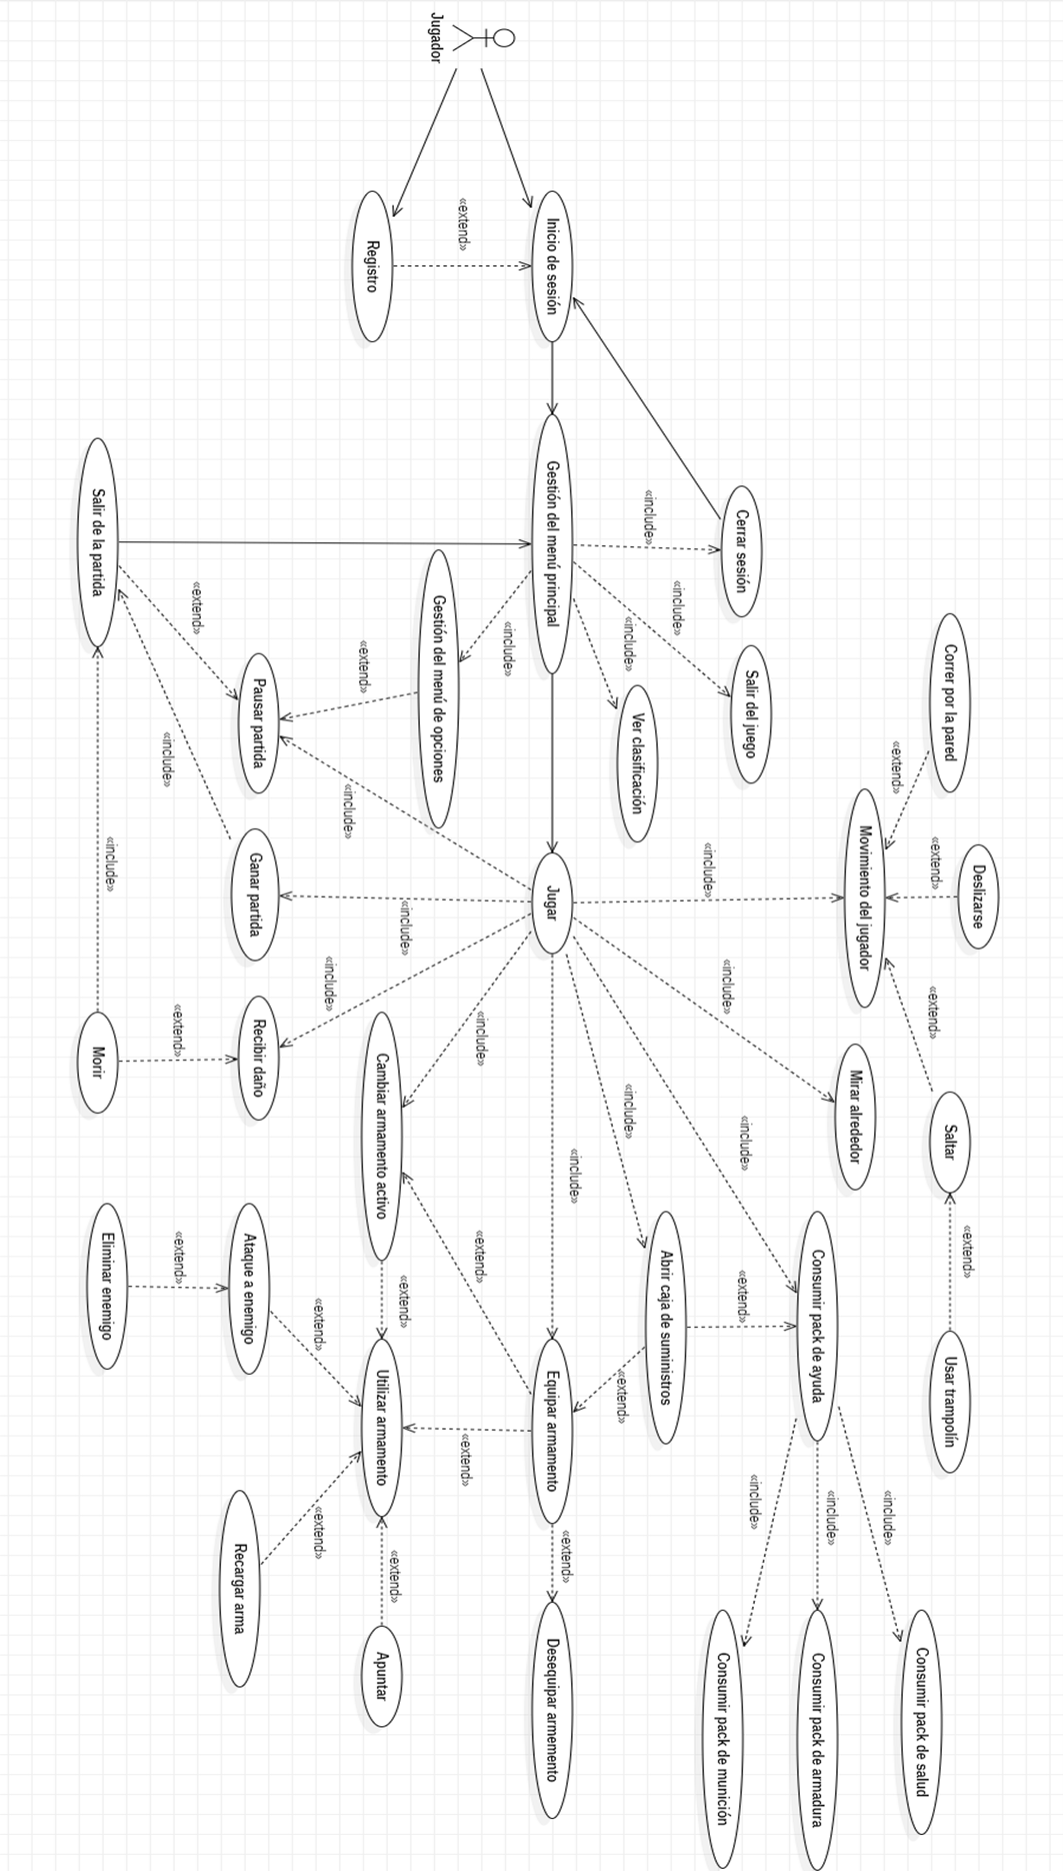
\includegraphics[scale=0.4]{img/UseCaseDiagram.png}
	\caption{Diagrama de casos de uso}
	\label{fig:CasosdeUso}
    \end{figure}
    
\subsection{Actores}
Al ser un videojuego en el que participa un solo jugador, el único actor del sistema será el propio jugador.

\subsection{Casos de Uso}
\tablaSmallSinColores{CU-01: Iniciar sesión}{p{3cm} p{.75cm} p{10cm}}{tablaCU1}{
	\multicolumn{3}{p{10.25cm}}{Caso de uso 1: Iniciar sesión} \\
}
{   
	Descripción                            & \multicolumn{2}{p{10.25cm}}{Permite al usuario de la aplicación identificarse de manera única e inequívoca para diferenciarse de los demás jugadores existentes y acceder a su cuenta.} \\\hline
	Requisitos                         	   & \multicolumn{2}{p{10.25cm}}{RF-1} \\\hline
	Precondiciones                         & \multicolumn{2}{p{10.25cm}}{Haber iniciado la aplicación y haber introducido las credenciales correctas del jugador} \\\hline

	\multirow{3}{2cm}{Secuencia normal}  & Paso & Acción \\\cline{2-3}
	& 1    & El usuario inicia el videojuego. \\\cline{2-3}
	& 2    & El usuario introduce sus credenciales (correo y contraseña). \\\cline{2-3}
	& 3    & El usuario pulsa en el botón ``Iniciar sesión''. \\\hline
	Postcondiciones                        & \multicolumn{2}{p{10.25cm}}{Se muestra el menú principal con algunos datos del usuario} \\\hline
	Excepciones                            & \multicolumn{2}{p{10.25cm}}{El usuario introduce las credenciales incorrectas, el sistema le avisa y puede introducirlas de nuevo. El usuario no está registrado. El usuario  sale de la aplicación.
}\\\hline
	Frecuencia                             & \multicolumn{2}{p{4cm}}{Baja} \\\hline
	Importancia                            & \multicolumn{2}{p{4cm}}{Muy alta} \\\hline

}
\tablaSmallSinColores{CU-2: Registrarse}{p{3cm} p{.75cm} p{10cm}}{tablaCU2}{
\multicolumn{3}{p{10.25cm}}{Caso de uso 2: Registrarse} \\
}
{   
Descripción                            & \multicolumn{2}{p{10.25cm}}{El usuario se da de alta en el juego para que empiece a registrar sus estadísticas} \\\hline
Requisitos                           & \multicolumn{2}{p{10.25cm}}{RF-1, RF-1-1} \\\hline
Precondiciones                         & \multicolumn{2}{p{10.25cm}}{Haber pulsado el botón “Registrarse” en la pantalla de identificación y haber introducido datos válidos} \\\hline

\multirow{3}{2cm}{Secuencia normal}  & Paso & Acción \\\cline{2-3}
& 1    & El usuario pulsa en “Registrarse”. \\\cline{2-3}
& 2    & El usuario introduce sus datos, como el nombre de usuario, el correo y la contraseña \\\cline{2-3}
& 3    & El usuario pulsa en “Registrarse”. \\\hline
Postcondiciones                        & \multicolumn{2}{p{10.25cm}}{El usuario puede iniciar sesión con su correo y contraseña} \\\hline
Excepciones                            & \multicolumn{2}{p{10.25cm}}{El usuario introduce algún dato inválido, el sistema le avisa y puede introducirlo de nuevo. El usuario vuelve a la pantalla de identificación sin terminar el registro}\\\hline
Frecuencia                             & \multicolumn{2}{p{4cm}}{Muy baja} \\\hline
Importancia                            & \multicolumn{2}{p{4cm}}{Muy alta} \\\hline

}


\tablaSmallSinColores{CU-3: Gestión del menú principal}{p{3cm} p{.75cm} p{10cm}}{tablaCU3}{
\multicolumn{3}{p{10.25cm}}{Caso de uso 3: Gestión del menú principal} \\
}
{   
Descripción                            & \multicolumn{2}{p{10.25cm}}{El usuario se encuentra en un menú donde puede escoger la acción que desee en relación con el juego, al tiempo que ve su nombre de usuario y su experiencia total actual} \\\hline
Requisitos                           & \multicolumn{2}{p{10.25cm}}{ RF-2, RF-2.1, RF-2.2, RF-2.3, RF-2.4, RF-2.5} \\\hline
Precondiciones                         & \multicolumn{2}{p{10.25cm}}{ El usuario debe haber iniciado sesión con éxito} \\\hline

\multirow{3}{2cm}{Secuencia normal}  & Paso & Acción \\\cline{2-3}
& 1    & El usuario accede al menú. \\\cline{2-3}
& 2    & El sistema muestra todas las acciones disponibles para el usuario. \\\cline{2-3}
& 3    & El usuario marca el botón de su elección. \\\cline{2-3}
& 4    & El sistema responde de acuerdo con la acción marcada \\\hline
Postcondiciones                        & \multicolumn{2}{p{10.25cm}}{Dependiendo de la opción elegida, el sistema tomará las acciones necesarias para responder la petición del usuario} \\\hline
Excepciones                            & \multicolumn{2}{p{10.25cm}}{El usuario pulsa la acción de “Salir” y la aplicación se cierra, terminando la secuencia del programa}\\\hline
Frecuencia                             & \multicolumn{2}{p{4cm}}{Baja} \\\hline
Importancia                            & \multicolumn{2}{p{4cm}}{Alta} \\\hline

}
\tablaSmallSinColores{CU-4: Jugar}{p{3cm} p{.75cm} p{10cm}}{tablaCU4}{
\multicolumn{3}{p{10.25cm}}{Caso de uso 4: Jugar} \\
}
{   
Descripción                            & \multicolumn{2}{p{10.25cm}}{El usuario selecciona la opción “jugar” en el menú principal para comenzar una partida} \\\hline
Requisitos                           & \multicolumn{2}{p{10.25cm}}{RF-3, RF-3.1, RF-3.2, RF-3.3, RF-3.4, RF-3.5, RF-3.6, RF-3.7, RF-3.8, RF-3.9, RF-3.10} \\\hline
Precondiciones                         & \multicolumn{2}{p{10.25cm}}{ El usuario debe haber pulsado el botón “Jugar” en el menú principal} \\\hline

\multirow{3}{2cm}{Secuencia normal}  & Paso & Acción \\\cline{2-3}
& 1    & El jugador pulsa “jugar” en el menú principal. \\\cline{2-3}
& 2    & El sistema muestra una pantalla de carga mientras construye el terreno y sus elementos. \\\cline{2-3}
& 3    & El jugador aparece en el mapa y puede empezar la partida. \\\hline
Postcondiciones                        & \multicolumn{2}{p{10.25cm}}{El jugador empieza la partida} \\\hline
Excepciones                            & \multicolumn{2}{p{10.25cm}}{-}\\\hline
Frecuencia                             & \multicolumn{2}{p{4cm}}{Baja} \\\hline
Importancia                            & \multicolumn{2}{p{4cm}}{Muy alta} \\\hline

}

\tablaSmallSinColores{CU-5: Movimiento del jugador}{p{3cm} p{.75cm} p{10cm}}{tablaCU5}{
\multicolumn{3}{p{10.25cm}}{Caso de uso 5: Movimiento del jugador} \\
}
{   
Descripción                            & \multicolumn{2}{p{10.25cm}}{El jugador se mueve por el terreno del mapa en la dirección deseada.} \\\hline
Requisitos                           & \multicolumn{2}{p{10.25cm}}{ RF-3, RF-3.2} \\\hline
Precondiciones                         & \multicolumn{2}{p{10.25cm}}{Haber comenzado una partida} \\\hline

\multirow{3}{2cm}{Secuencia normal}  & Paso & Acción \\\cline{2-3}
& 1    & El usuario presiona las teclas “W” (adelante), “S” (atrás), “A” (izquierda) o “D” (Derecha), según la dirección en la que se quiera mover. Opcionalmente puede mantener pulsada la tecla “shift” para correr. \\\hline
Postcondiciones                        & \multicolumn{2}{p{10.25cm}}{El jugador se desplaza hacia un determinada dirección según las teclas pulsadas.} \\\hline
Excepciones                            & \multicolumn{2}{p{10.25cm}}{El usuario no presiona ninguna tecla y el jugador no se mueve}\\\hline
Frecuencia                             & \multicolumn{2}{p{4cm}}{Muy alta } \\\hline
Importancia                            & \multicolumn{2}{p{4cm}}{Alta} \\\hline

}
\tablaSmallSinColores{CU-6: Deslizarse}{p{3cm} p{.75cm} p{10cm}}{tablaCU6}{
\multicolumn{3}{p{10.25cm}}{Caso de uso 6: Deslizarse} \\
}
{   
Descripción                            & \multicolumn{2}{p{10.25cm}}{El jugador se desliza por el terreno cuando está lo suficientemente inclinado} \\\hline
Requisitos                           & \multicolumn{2}{p{10.25cm}}{RF-3, RF-3.2, RF-3.2.1} \\\hline
Precondiciones                         & \multicolumn{2}{p{10.25cm}}{ El jugador tiene los pies apoyados sobre el suelo} \\\hline

\multirow{3}{2cm}{Secuencia normal}  & Paso & Acción \\\cline{2-3}
& 1    & El usuario presiona la tecla “Ctrl” (Control) y opcionalmente también alguna tecla de dirección para dirigir mejor el movimiento. \\\cline{2-3}
& 2    & El jugador, si se encuentra sobre un terreno inclinado hacia abajo, se desliza por él. \\\hline
Postcondiciones                        & \multicolumn{2}{p{10.25cm}}{El jugador se desplaza rápidamente hacia una zona más baja del mapa} \\\hline
Excepciones                            & \multicolumn{2}{p{10.25cm}}{No hay suficiente pendiente para deslizarse }\\\hline
Frecuencia                             & \multicolumn{2}{p{4cm}}{Media } \\\hline
Importancia                            & \multicolumn{2}{p{4cm}}{Media} \\\hline

}
\tablaSmallSinColores{CU-7: Correr por la pared}{p{3cm} p{.75cm} p{10cm}}{tablaCU7}{
\multicolumn{3}{p{10.25cm}}{Caso de uso 7: Correr por la pared} \\
}
{   
Descripción                            & \multicolumn{2}{p{10.25cm}}{El jugador puede adherirse a una pared para correr sobre ella y saltar desde la pared a otras paredes cercanas, creando un efecto de escalada alterno.} \\\hline
Requisitos                           & \multicolumn{2}{p{10.25cm}}{RF-3, RF-3.2, RF-3.2.2} \\\hline
Precondiciones                         & \multicolumn{2}{p{10.25cm}}{Debe haber una pared junto al jugador} \\\hline

\multirow{3}{2cm}{Secuencia normal}  & Paso & Acción \\\cline{2-3}
& 1    & El usuario salta junto a una pared. \\\cline{2-3}
& 2    & El jugador automáticamente se adhiere a dicha pared. \\\cline{2-3}
& 3    & Mientras tenga la tecla de dirección que apunta a la pared presionada, el jugador se mantiene adherido. \\\cline{2-3}
& 4    & El jugador presiona avanza por la pared presionando la tecla de dirección “W”. \\\cline{2-3}
& 5    & El jugador puede saltar en dirección opuesta a la pared presionando la tecla de salto “Espacio” y poder alcanzar un sitio más alto \\\hline
Postcondiciones                        & \multicolumn{2}{p{10.25cm}}{El jugador puede repetir esta acción en paredes cercanas para crear un efecto de escalada} \\\hline
Excepciones                            & \multicolumn{2}{p{10.25cm}}{ El usuario deja de presionar la tecla de dirección correcta y se baja de la pared}\\\hline
Frecuencia                             & \multicolumn{2}{p{4cm}}{Media} \\\hline
Importancia                            & \multicolumn{2}{p{4cm}}{Media} \\\hline

}
\tablaSmallSinColores{CU-8: Mirar alrededor }{p{3cm} p{.75cm} p{10cm}}{tablaCU8}{
\multicolumn{3}{p{10.25cm}}{Caso de uso 8: Mirar alrededor} \\
}
{   
Descripción                            & \multicolumn{2}{p{10.25cm}}{El jugador gira su cabeza para mirar el entorno y los objetos de su alrededor} \\\hline
Requisitos                           & \multicolumn{2}{p{10.25cm}}{RF-3, RF-3.3} \\\hline
Precondiciones                         & \multicolumn{2}{p{10.25cm}}{Haber comenzado una partida} \\\hline

\multirow{3}{2cm}{Secuencia normal}  & Paso & Acción \\\cline{2-3}
& 1    & El usuario desplaza el ratón en la dirección hacia la que quiera dirigir la mirada del jugador. \\\cline{2-3}
& 2    & El jugador gira su cabeza. \\\hline
Postcondiciones                        & \multicolumn{2}{p{10.25cm}}{El jugador puede ver la parte del entorno correspondiente} \\\hline
Excepciones                            & \multicolumn{2}{p{10.25cm}}{ El jugador no mueve el ratón y siempre verá la misma región}\\\hline
Frecuencia                             & \multicolumn{2}{p{4cm}}{Muy alta} \\\hline
Importancia                            & \multicolumn{2}{p{4cm}}{Alta} \\\hline

}
\tablaSmallSinColores{CU-9: Salto del jugador}{p{3cm} p{.75cm} p{10cm}}{tablaCU9}{
\multicolumn{3}{p{10.25cm}}{Caso de uso 9: Salto del jugador} \\
}
{   
Descripción                            & \multicolumn{2}{p{10.25cm}}{El jugador se eleva en el aire unos instantes} \\\hline
Requisitos                           & \multicolumn{2}{p{10.25cm}}{RF-3, RF-3.4} \\\hline
Precondiciones                         & \multicolumn{2}{p{10.25cm}}{El jugador tiene los pies apoyados en alguna superficie} \\\hline

\multirow{3}{2cm}{Secuencia normal}  & Paso & Acción \\\cline{2-3}
& 1    & El usuario presiona la tecla “Espacio”. \\\cline{2-3}
& 2    & El jugador salta. \\\hline
Postcondiciones                        & \multicolumn{2}{p{10.25cm}}{El jugador vuelve a caer por el efecto de la gravedad.} \\\hline
Excepciones                            & \multicolumn{2}{p{10.25cm}}{ El jugador ya se encuentra en el aire}\\\hline
Frecuencia                             & \multicolumn{2}{p{4cm}}{Media} \\\hline
Importancia                            & \multicolumn{2}{p{4cm}}{Baja} \\\hline

}
\tablaSmallSinColores{CU-10: Usar trampolín}{p{3cm} p{.75cm} p{10cm}}{tablaCU10}{
\multicolumn{3}{p{10.25cm}}{Caso de uso 10: Usar trampolín} \\
}
{   
Descripción                            & \multicolumn{2}{p{10.25cm}}{El jugador se impulsa varios metros en el aire, haciendo que pueda alcanzar lugares muy altos o que pueda escapar de algún sitio rápidamente} \\\hline
Requisitos                           & \multicolumn{2}{p{10.25cm}}{RF-3, RF-3.4, RF-3.4.1} \\\hline
Precondiciones                         & \multicolumn{2}{p{10.25cm}}{El jugador tiene se encuentra sobre una plataforma de salto} \\\hline

\multirow{3}{2cm}{Secuencia normal}  & Paso & Acción \\\cline{2-3}
& 1    & El usuario se sitúa sobre una plataforma de salto. \\\cline{2-3}
& 2    & El usuario presiona la tecla “Espacio”. \\\cline{2-3}
& 3    & El sistema eleva al jugador varios metros en el aire. \\\hline
Postcondiciones                        & \multicolumn{2}{p{10.25cm}}{El jugador vuelve a caer por el efecto de la gravedad} \\\hline
Excepciones                            & \multicolumn{2}{p{10.25cm}}{El jugador ya se encuentra en el aire}\\\hline
Frecuencia                             & \multicolumn{2}{p{4cm}}{Media-baja} \\\hline
Importancia                            & \multicolumn{2}{p{4cm}}{Baja} \\\hline

}
\tablaSmallSinColores{CU-11: Abrir caja de suministros}{p{3cm} p{.75cm} p{10cm}}{tablaCU11}{
\multicolumn{3}{p{10.25cm}}{Caso de uso 11: Abrir caja de suministros} \\
}
{   
Descripción                            & \multicolumn{2}{p{10.25cm}}{El jugador abre una caja de suministros que encuentre, que contiene diferentes tipos de objetos que le pueden ayudar} \\\hline
Requisitos                           & \multicolumn{2}{p{10.25cm}}{RF-3, RF-3.5} \\\hline
Precondiciones                         & \multicolumn{2}{p{10.25cm}}{El jugador dirige su mirada hacia una caja de suministros cercana a él} \\\hline

\multirow{3}{2cm}{Secuencia normal}  & Paso & Acción \\\cline{2-3}
& 1    & El sistema, si se da el caso, avisa al jugador por medio de un texto de que puede abrir la caja correspondiente pulsando la tecla de interacción “E”. \\\cline{2-3}
& 2    & El jugador pulsa la tecla de interacción y la caja se abre. \\\hline
Postcondiciones                        & \multicolumn{2}{p{10.25cm}}{Se generan 4 objetos aleatorios, como armas, granadas o packs de ayuda.} \\\hline
Excepciones                            & \multicolumn{2}{p{10.25cm}}{La caja ya ha sido abierta}\\\hline
Frecuencia                             & \multicolumn{2}{p{4cm}}{Media-baja} \\\hline
Importancia                            & \multicolumn{2}{p{4cm}}{Media} \\\hline

}
\tablaSmallSinColores{CU-12: Equipar armamento}{p{3cm} p{.75cm} p{10cm}}{tablaCU12}{
\multicolumn{3}{p{10.25cm}}{Caso de uso 12: Equipar armamento} \\
}
{   
Descripción                            & \multicolumn{2}{p{10.25cm}}{El jugador añade a su inventario un arma o granada que encuentre} \\\hline
Requisitos                           & \multicolumn{2}{p{10.25cm}}{RF-3, RF-3.6, RF-3.14} \\\hline
Precondiciones                         & \multicolumn{2}{p{10.25cm}}{Dirigir la mirada hacia un arma o granada cercana} \\\hline

\multirow{3}{2cm}{Secuencia normal}  & Paso & Acción \\\cline{2-3}
& 1    & El sistema, si se da el caso, avisa al jugador por medio de un texto de que puede equipar el armamento en cuestión pulsando la tecla de interacción “E”. \\\cline{2-3}
& 2    & El jugador pulsa la tecla de interacción. \\\cline{2-3}
& 3    & El armamento correspondiente se añade al inventario del jugador. \\\hline
Postcondiciones                        & \multicolumn{2}{p{10.25cm}}{El jugador puede utilizar el armamento equipado} \\\hline
Excepciones                            & \multicolumn{2}{p{10.25cm}}{El inventario está lleno, entonces el nuevo objeto sustituirá al objeto que estuviera equipado en esa celda del inventario}\\\hline
Frecuencia                             & \multicolumn{2}{p{4cm}}{Media} \\\hline
Importancia                            & \multicolumn{2}{p{4cm}}{Media-alta} \\\hline

}
\tablaSmallSinColores{CU-13: Desequipar armamento}{p{3cm} p{.75cm} p{10cm}}{tablaCU13}{
\multicolumn{3}{p{10.25cm}}{Caso de uso 13: Desequipar armamento } \\
}
{   
Descripción                            & \multicolumn{2}{p{10.25cm}}{El jugador suelta un objeto que no quiera tener más tiempo en su inventario.} \\\hline
Requisitos                           & \multicolumn{2}{p{10.25cm}}{RF-3, RF-3.7} \\\hline
Precondiciones                         & \multicolumn{2}{p{10.25cm}}{Tener un objeto en el espacio activo del inventario} \\\hline

\multirow{3}{2cm}{Secuencia normal}  & Paso & Acción \\\cline{2-3}
& 1    & El jugador presiona la tecla “Q” una vez (También puede ocurrir que el jugador equipe un objeto y el inventario esté lleno, haciendo que se desequipe el objeto que se encuentre en la celda activa del inventario). \\\hline
Postcondiciones                        & \multicolumn{2}{p{10.25cm}}{El objeto en cuestión deja de estar equipado y se deja sobre el suelo. La celda del inventario donde estaba se vacía.} \\\hline
Excepciones                            & \multicolumn{2}{p{10.25cm}}{La celda activa del inventario ya está vacía}\\\hline
Frecuencia                             & \multicolumn{2}{p{4cm}}{Media} \\\hline
Importancia                            & \multicolumn{2}{p{4cm}}{Media-baja} \\\hline

}
\tablaSmallSinColores{CU-14: Cambiar armamento activo}{p{3cm} p{.75cm} p{10cm}}{tablaCU14}{
\multicolumn{3}{p{10.25cm}}{Caso de uso 14: Cambiar armamento activo} \\
}
{   
Descripción                            & \multicolumn{2}{p{10.25cm}}{El jugador selecciona qué objeto del inventario desea tener activo y listo para usar.} \\\hline
Requisitos                           & \multicolumn{2}{p{10.25cm}}{RF-3, RF-3.8, RF-3.14} \\\hline
Precondiciones                         & \multicolumn{2}{p{10.25cm}}{Haber iniciado una partida} \\\hline

\multirow{3}{2cm}{Secuencia normal}  & Paso & Acción \\\cline{2-3}
& 1    & El jugador gira la rueda del ratón hasta tener activa la celda del inventario que contiene el objeto deseado. \\\hline
Postcondiciones                        & \multicolumn{2}{p{10.25cm}}{El objeto que el jugador puede usar se actualiza al deseado.} \\\hline
Excepciones                            & \multicolumn{2}{p{10.25cm}}{La celda objetivo del inventario está vacía, por lo que ningún objeto estará listo para usarse}\\\hline
Frecuencia                             & \multicolumn{2}{p{4cm}}{Alta} \\\hline
Importancia                            & \multicolumn{2}{p{4cm}}{Alta} \\\hline

}
\tablaSmallSinColores{CU-15: Utilizar armamento}{p{3cm} p{.75cm} p{10cm}}{tablaCU15}{
\multicolumn{3}{p{10.25cm}}{Caso de uso 15: Utilizar armamento } \\
}
{   
Descripción                            & \multicolumn{2}{p{10.25cm}}{El jugador dispara con el arma activa, o lanza la granada activa, generalmente para intentar acertar en los enemigos, y así poder eliminarlos.} \\\hline
Requisitos                           & \multicolumn{2}{p{10.25cm}}{RF-3, RF-3.9, RF-9.1, RF-9.2, RF-3.14} \\\hline
Precondiciones                         & \multicolumn{2}{p{10.25cm}}{Tener algún arma o granada activa en el inventario y munición disponible} \\\hline

\multirow{3}{2cm}{Secuencia normal}  & Paso & Acción \\\cline{2-3}
& 1    & El jugador presiona el clic izquierdo del ratón de manera unitaria o continua, dependiendo de las características del armamento activo, como el tipo de arma o su rareza (Común, rara, épica, legendaria). \\\hline
Postcondiciones                        & \multicolumn{2}{p{10.25cm}}{El armamento responde lanzando “balas” o la granada en sí.} \\\hline
Excepciones                            & \multicolumn{2}{p{10.25cm}}{La celda del inventario activa está vacía o el armamento no tiene munición restante}\\\hline
Frecuencia                             & \multicolumn{2}{p{4cm}}{Muy alta} \\\hline
Importancia                            & \multicolumn{2}{p{4cm}}{Muy alta} \\\hline

}
\tablaSmallSinColores{CU-16: Recargar arma}{p{3cm} p{.75cm} p{10cm}}{tablaCU16}{
\multicolumn{3}{p{10.25cm}}{Caso de uso 16: Recargar arma} \\
}
{   
Descripción                            & \multicolumn{2}{p{10.25cm}}{El jugador recarga el arma actual para tener más munición preparada.} \\\hline
Requisitos                           & \multicolumn{2}{p{10.25cm}}{RF-3, RF-3.9, RF-3.9.3, RF-3.14} \\\hline
Precondiciones                         & \multicolumn{2}{p{10.25cm}}{Tener un arma activa en el inventario y munición en la reserva} \\\hline

\multirow{3}{2cm}{Secuencia normal}  & Paso & Acción \\\cline{2-3}
& 1    & El jugador presiona la tecla “R” para recargar el arma. \\\hline
Postcondiciones                        & \multicolumn{2}{p{10.25cm}}{El arma llena su cargador actual. La munición de reserva del arma disminuye. Se actualizan los valores del HUD correspondientes a la munición del arma actual.} \\\hline
Excepciones                            & \multicolumn{2}{p{10.25cm}}{El arma ya tiene el cargador actual completo}\\\hline
Frecuencia                             & \multicolumn{2}{p{4cm}}{Alta} \\\hline
Importancia                            & \multicolumn{2}{p{4cm}}{Media-alta} \\\hline

}
\tablaSmallSinColores{CU-17: Apuntar}{p{3cm} p{.75cm} p{10cm}}{tablaCU17}{
\multicolumn{3}{p{10.25cm}}{Caso de uso 17: Apuntar} \\
}
{   
Descripción                            & \multicolumn{2}{p{10.25cm}}{El jugador apunta con el armamento actual para tener más precisión antes de disparar.} \\\hline
Requisitos                           & \multicolumn{2}{p{10.25cm}}{ RF-3, RF-3.9, RF-3.9.4} \\\hline
Precondiciones                         & \multicolumn{2}{p{10.25cm}}{Tener algún arma o granada activa en el inventario} \\\hline

\multirow{3}{2cm}{Secuencia normal}  & Paso & Acción \\\cline{2-3}
& 1    & El jugador presiona el clic derecho del ratón tanto tiempo que quiera apuntar con el armamento activo. \\\hline
Postcondiciones                        & \multicolumn{2}{p{10.25cm}}{Disminuye el campo de visión de la cámara haciendo un efecto de “zoom”, y se disminuye la sensibilidad del ratón, haciendo que el jugador tenga más precisión} \\\hline
Excepciones                            & \multicolumn{2}{p{10.25cm}}{-}\\\hline
Frecuencia                             & \multicolumn{2}{p{4cm}}{Media} \\\hline
Importancia                            & \multicolumn{2}{p{4cm}}{Media} \\\hline

}
\tablaSmallSinColores{CU-18: Consumir packs de ayuda}{p{3cm} p{.75cm} p{10cm}}{tablaCU18}{
\multicolumn{3}{p{10.25cm}}{Caso de uso 18: Consumir packs de ayuda} \\
}
{   
Descripción                            & \multicolumn{2}{p{10.25cm}}{El jugador puede consumir diferentes paquetes de ayuda que se encuentre por el mapa y que le otorgan diferentes ayudas para mantenerse con vida} \\\hline
Requisitos                           & \multicolumn{2}{p{10.25cm}}{RF-3, RF-3.10, RF-3.14} \\\hline
Precondiciones                         & \multicolumn{2}{p{10.25cm}}{Encontrar algún pack de ayuda en el mapa, bien a través de cajas de suministro o porque algún enemigo lo haya soltado} \\\hline

\multirow{3}{2cm}{Secuencia normal}  & Paso & Acción \\\cline{2-3}
& 1    & El jugador se encuentra un pack de ayuda cercano. \\\cline{2-3}
& 2    & El jugador dirige la mirada hacia el pack de ayuda. \\\cline{2-3}
& 3    & El jugador presiona la tecla de interacción para consumirlo. \\\hline
Postcondiciones                        & \multicolumn{2}{p{10.25cm}}{El jugador recibe algún efecto beneficioso para ayudarlo en la partida, como más salud, más armadura o más munición} \\\hline
Excepciones                            & \multicolumn{2}{p{10.25cm}}{- }\\\hline
Frecuencia                             & \multicolumn{2}{p{4cm}}{Media} \\\hline
Importancia                            & \multicolumn{2}{p{4cm}}{Media} \\\hline

}
\tablaSmallSinColores{CU-19: Consumir pack de salud}{p{3cm} p{.75cm} p{10cm}}{tablaCU19}{
\multicolumn{3}{p{10.25cm}}{Caso de uso 19: Consumir pack de salud} \\
}
{   
Descripción                            & \multicolumn{2}{p{10.25cm}}{El jugador consume un pack de salud que encuentre para recuperar algo de vida} \\\hline
Requisitos                           & \multicolumn{2}{p{10.25cm}}{RF-3, RF-3.10, RF-3.10.1, RF-3.14} \\\hline
Precondiciones                         & \multicolumn{2}{p{10.25cm}}{El jugador debe dirigir la mirada hacia un pack de salud cercano} \\\hline

\multirow{3}{2cm}{Secuencia normal}  & Paso & Acción \\\cline{2-3}
& 1    & El sistema, si se da el caso, avisa al jugador por medio de un texto de que puede recuperar cierta cantidad de salud si presiona la tecla de interacción “E”.\\\cline{2-3}
& 2    & El jugador pulsa la tecla de interacción y recupera determinados puntos de salud en función de la rareza del pack (Común +25, Raro +50, Épico +75, Legendario +100).\\\hline
Postcondiciones                        & \multicolumn{2}{p{10.25cm}}{ El jugador recupera salud y la barra de vida del HUD se actualiza.} \\\hline
Excepciones                            & \multicolumn{2}{p{10.25cm}}{No tiene efecto si el jugador ya tiene la salud al máximo}\\\hline
Frecuencia                             & \multicolumn{2}{p{4cm}}{Media-baja} \\\hline
Importancia                            & \multicolumn{2}{p{4cm}}{Media} \\\hline

}

\tablaSmallSinColores{CU-20: Consumir pack de armadura}{p{3cm} p{.75cm} p{10cm}}{tablaCU20}{
	\multicolumn{3}{p{10.25cm}}{Caso de uso 20: Consumir pack de armadura} \\
}
{   
	Descripción                            & \multicolumn{2}{p{10.25cm}}{El jugador consume un pack de armadura que encuentre para recuperar algo de armadura.} \\\hline
	Requisitos                         	   & \multicolumn{2}{p{10.25cm}}{RF-3, RF-3.10, RF-3.10.2, RF-3.14} \\\hline
	Precondiciones                         & \multicolumn{2}{p{10.25cm}}{El jugador debe dirigir la mirada hacia un pack de armadura cercano} \\\hline

	\multirow{3}{2cm}{Secuencia normal}  & Paso & Acción \\\cline{2-3}
	& 1    & El sistema, si se da el caso, avisa al jugador por medio de un texto de que puede recuperar cierta cantidad de armadura si presiona la tecla de interacción “E” \\\cline{2-3}
	& 2    & El jugador pulsa la tecla de interacción y recupera determinados puntos de armadura en función de la rareza del pack (Común +25, Raro +50, Épico +75, Legendario +100)\\\hline
	Postcondiciones                        & \multicolumn{2}{p{10.25cm}}{El jugador recupera armadura y la barra de armadura del HUD se actualiza} \\\hline
	Excepciones                            & \multicolumn{2}{p{10.25cm}}{No tiene efecto si el jugador ya tiene los puntos de armadura al máximo}\\\hline
	Frecuencia                             & \multicolumn{2}{p{4cm}}{Media-baja} \\\hline
	Importancia                            & \multicolumn{2}{p{4cm}}{Media} \\\hline

}
\tablaSmallSinColores{CU-21: Consumir pack de munición}{p{3cm} p{.75cm} p{10cm}}{tablaCU21}{
	\multicolumn{3}{p{10.25cm}}{Caso de uso 21: Consumir pack de munición} \\
}
{   
	Descripción                            & \multicolumn{2}{p{10.25cm}}{El jugador consume un pack de munición que encuentre para rellenar la munición de las armas equipadas.} \\\hline
	Requisitos                         	   & \multicolumn{2}{p{10.25cm}}{RF-3, RF-3.10, RF-3.10.3, RF-3.14} \\\hline
	Precondiciones                         & \multicolumn{2}{p{10.25cm}}{El jugador debe dirigir la mirada hacia un pack de munición cercano} \\\hline

	\multirow{3}{2cm}{Secuencia normal}  & Paso & Acción \\\cline{2-3}
	& 1    & El sistema, si se da el caso, avisa al jugador por medio de un texto de que puede obtener cierta cantidad de munición si presiona la tecla de interacción “E”. \\\cline{2-3}
	& 2    & El jugador pulsa la tecla de interacción y obtiene tantos cargadores de munición de cada arma equipada en función de la rareza del pack (Común +1 cargador, Raro +2 cargadores, Épico +3 cargadores, Legendario +4 cargadores)\\\hline
	Postcondiciones                        & \multicolumn{2}{p{10.25cm}}{Las armas equipadas reciben cargadores y los valores correspondientes del HUD se actualizan } \\\hline
	Excepciones                            & \multicolumn{2}{p{10.25cm}}{No tiene efecto si el jugador no tiene ningún arma equipada en el inventario.}\\\hline
	Frecuencia                             & \multicolumn{2}{p{4cm}}{Media-baja} \\\hline
	Importancia                            & \multicolumn{2}{p{4cm}}{Media} \\\hline

}
\tablaSmallSinColores{CU-22: Recibir daño}{p{3cm} p{.75cm} p{10cm}}{tablaCU22}{
	\multicolumn{3}{p{10.25cm}}{Caso de uso 22: Recibir daño} \\
}
{   
	Descripción                            & \multicolumn{2}{p{10.25cm}}{El jugador recibe daño de alguna fuente y su armadura y/o salud disminuyen} \\\hline
	Requisitos                         	   & \multicolumn{2}{p{10.25cm}}{RF-3, RF-3.12, RF-3.13, RF-3.14} \\\hline
	Precondiciones                         & \multicolumn{2}{p{10.25cm}}{Algún elemento o entidad hace daño al jugador de alguna manera} \\\hline

	\multirow{3}{2cm}{Secuencia normal}  & Paso & Acción \\\cline{2-3}
	& 1    & El jugador recibe daño de alguna manera (Un enemigo dispara al jugador, una granada explosiva explota cerca del jugador, la nube tóxica alcanza al jugador)\\\cline{2-3}
	& 2    & Se muestra un indicador visual para que el jugador sepa desde qué dirección está recibiendo el daño \\\hline
	Postcondiciones                        & \multicolumn{2}{p{10.25cm}}{La armadura y/o salud del jugador disminuye, y la interfaz de usuario reacciona acorde, mostrando efectos de daño, sonidos y estremeciéndose la cámara en función del daño recibido.} \\\hline
	Excepciones                            & \multicolumn{2}{p{10.25cm}}{Si el jugador ya ha muerto, no recibe daño}\\\hline
	Frecuencia                             & \multicolumn{2}{p{4cm}}{media} \\\hline
	Importancia                            & \multicolumn{2}{p{4cm}}{Muy alta} \\\hline

}
\tablaSmallSinColores{CU-23: Ataque a enemigo}{p{3cm} p{.75cm} p{10cm}}{tablaCU23}{
	\multicolumn{3}{p{10.25cm}}{Caso de uso 23: Ataque a enemigo} \\
}
{   
	Descripción                            & \multicolumn{2}{p{10.25cm}}{Los enemigos reciben daño si el jugador le dispara con algún arma o si le alcanza con una granada explosiva} \\\hline
	Requisitos                         	   & \multicolumn{2}{p{10.25cm}}{RF-3, RF-3.11, RF-3.11.2} \\\hline
	Precondiciones                         & \multicolumn{2}{p{10.25cm}}{El enemigo se encuentra dentro del alcance de ataque del jugador} \\\hline

	\multirow{3}{2cm}{Secuencia normal}  & Paso & Acción \\\cline{2-3}
	& 1    & El jugador dispara y su mirilla está alineada con el enemigo o le alcanza con una granada explosiva. \\\cline{2-3}
	& 2    & El enemigo se estremece y pierde parte de sus puntos de armadura y/o salud en función del arma con la que se le ataque. \\\cline{2-3}
	& 3    & Aparece un texto flotante con la cantidad de daño infligido sobre la cabeza del enemigo \\\hline
	Postcondiciones                        & \multicolumn{2}{p{10.25cm}}{La vida del enemigo y las balas del arma correspondiente disminuyen, la barra de salud del enemigo se actualiza} \\\hline
	Excepciones                            & \multicolumn{2}{p{10.25cm}}{El jugador se encuentra demasiado lejos del enemigo
}\\\hline
	Frecuencia                             & \multicolumn{2}{p{4cm}}{Alta} \\\hline
	Importancia                            & \multicolumn{2}{p{4cm}}{Alta} \\\hline

}
\tablaSmallSinColores{CU-24: Eliminar enemigo}{p{3cm} p{.75cm} p{10cm}}{tablaCU24}{
	\multicolumn{3}{p{10.25cm}}{Caso de uso 24: Eliminar enemigo} \\
}
{   
	Descripción                            & \multicolumn{2}{p{10.25cm}}{El jugador elimina a un enemigo} \\\hline
	Requisitos                         	   & \multicolumn{2}{p{10.25cm}}{RF-3, RF-3.11, RF-3.11.2, RF-3.11.3, RF-3.14} \\\hline
	Precondiciones                         & \multicolumn{2}{p{10.25cm}}{El enemigo se encuentra dentro del alcance de ataque del jugador} \\\hline

	\multirow{3}{2cm}{Secuencia normal}  & Paso & Acción \\\cline{2-3}
	& 1    & El jugador dispara y su mirilla está alineada con el enemigo, o le alcanza con una granada explosiva. \\\cline{2-3}
	& 2    & El enemigo pierde más puntos de vida que los que le quedan. \\\cline{2-3}
	& 3    & El enemigo muere \\\hline
	Postcondiciones                        & \multicolumn{2}{p{10.25cm}}{Disminuye el contador de entidades vivas en la partida. Aumenta el contador de enemigos eliminados por el jugador. El enemigo suelta varios objetos de ayuda para el jugador a modo de recompensa.
} \\\hline
	Excepciones                            & \multicolumn{2}{p{10.25cm}}{-}\\\hline
	Frecuencia                             & \multicolumn{2}{p{4cm}}{Media} \\\hline
	Importancia                            & \multicolumn{2}{p{4cm}}{Alta} \\\hline

}
\tablaSmallSinColores{CU-25: Pausar partida}{p{3cm} p{.75cm} p{10cm}}{tablaCU25}{
	\multicolumn{3}{p{10.25cm}}{Caso de uso 25: Pausar partida} \\
}
{   
	Descripción                            & \multicolumn{2}{p{10.25cm}}{La partida queda congelada y se le ofrecen distintas opciones al jugador, concretamente reanudar la partida, modificar las opciones o salir al menú} \\\hline
	Requisitos                         	   & \multicolumn{2}{p{10.25cm}}{RF-3, RF-3.15} \\\hline
	Precondiciones                         & \multicolumn{2}{p{10.25cm}}{Haber iniciado una partida} \\\hline

	\multirow{3}{2cm}{Secuencia normal}  & Paso & Acción \\\cline{2-3}
	& 1    & El jugador presiona la tecla “Esc” (Escape) una vez \\\cline{2-3}
	& 2    & El videojuego se pausa \\\cline{2-3}
	& 3    & Se le ofrecen al usuario las acciones de continuar, ver el menú de opciones o salir de la partida. \\\cline{2-3}
	& 4    & El sistema espera a la espera de una acción del usuario\\\hline
	Postcondiciones                        & \multicolumn{2}{p{10.25cm}}{Se reanuda el juego o se abre el menú de opciones antes de volver al juego} \\\hline
	Excepciones                            & \multicolumn{2}{p{10.25cm}}{El jugador presiona el botón “salir” haciendo que se termine la partida inmediatamente y se vuelva al menú principal}\\\hline
	Frecuencia                             & \multicolumn{2}{p{4cm}}{Baja} \\\hline
	Importancia                            & \multicolumn{2}{p{4cm}}{Baja} \\\hline

}
\tablaSmallSinColores{CU-26: Gestión del menú de opciones}{p{3cm} p{.75cm} p{10cm}}{tablaCU26}{
	\multicolumn{3}{p{10.25cm}}{Caso de uso 26: Gestión del menú de opciones} \\
}
{   
	Descripción                            & \multicolumn{2}{p{10.25cm}}{Permitir al usuario modificar alguna característica general del juego, como el volumen, la resolución o la calidad gráfica, tanto en el menú principal como una vez iniciada la partida.} \\\hline
	Requisitos                         	   & \multicolumn{2}{p{10.25cm}}{RF-2, RF-2.2} \\\hline
	Precondiciones                         & \multicolumn{2}{p{10.25cm}}{Escoger la acción “opciones” en el menú} \\\hline

	\multirow{3}{2cm}{Secuencia normal}  & Paso & Acción \\\cline{2-3}
	& 1    & El sistema muestra al jugador una serie de opciones a modificar.\\\cline{2-3}
	& 2    & El jugador se desplaza hasta la que desee modificar\\\cline{2-3}
	& 3    & El jugador modifica la característica elegida\\\cline{2-3}
	& 4    & El jugador presiona el botón “hecho” para guardar los cambios y salir del menú de opciones \\\hline
	Postcondiciones                        & \multicolumn{2}{p{10.25cm}}{Algún aspecto del videojuego se modifica en función de la opción elegida por el jugador} \\\hline
	Excepciones                            & \multicolumn{2}{p{10.25cm}}{-}\\\hline
	Frecuencia                             & \multicolumn{2}{p{4cm}}{Media-Baja} \\\hline
	Importancia                            & \multicolumn{2}{p{4cm}}{Media-Alta} \\\hline

}
\tablaSmallSinColores{CU-27: Salir de la partida}{p{3cm} p{.75cm} p{10cm}}{tablaCU27}{
	\multicolumn{3}{p{10.25cm}}{Caso de uso 27: Salir de la partida} \\
}
{   
	Descripción                            & \multicolumn{2}{p{10.25cm}}{El jugador vuelve al menú principal del juego.} \\\hline
	Requisitos                         	   & \multicolumn{2}{p{10.25cm}}{RF-2, RF-3.16} \\\hline
	Precondiciones                         & \multicolumn{2}{p{10.25cm}}{El jugador debe tener disponible el botón “Salir” en el menú actual} \\\hline

	\multirow{3}{2cm}{Secuencia normal}  & Paso & Acción \\\cline{2-3}
	& 1    & El jugador, o bien se encuentra en el menú de pausa, o muere, o gana la partida \\\cline{2-3}
	& 2    & El jugador pulsa el botón “salir” \\\cline{2-3}
	& 3    & Si ha ganado o perdido la partida, se actualiza su experiencia en la base de datos \\\hline
	Postcondiciones                        & \multicolumn{2}{p{10.25cm}}{La partida finaliza y el usuario viaja al menú principal} \\\hline
	Excepciones                            & \multicolumn{2}{p{10.25cm}}{Si el jugador sale desde el menú de pausa, no se actualiza su experiencia ganada en la partida.}\\\hline
	Frecuencia                             & \multicolumn{2}{p{4cm}}{Baja} \\\hline
	Importancia                            & \multicolumn{2}{p{4cm}}{Alta} \\\hline

}
\tablaSmallSinColores{CU-28: Ganar partida}{p{3cm} p{.75cm} p{10cm}}{tablaCU28}{
	\multicolumn{3}{p{10.25cm}}{Caso de uso 28: Ganar partida} \\
}
{   
	Descripción                            & \multicolumn{2}{p{10.25cm}}{El jugador consigue la victoria al quedar como único superviviente de la partida.} \\\hline
	Requisitos                         	   & \multicolumn{2}{p{10.25cm}}{RF-3, RF-3.14, RF-3.17} \\\hline
	Precondiciones                         & \multicolumn{2}{p{10.25cm}}{Todos los enemigos deben haber sido eliminados} \\\hline

	\multirow{3}{2cm}{Secuencia normal}  & Paso & Acción \\\cline{2-3}
	& 1    & El jugador junto, junto al resto de enemigos, consigue acabar con todos los enemigos de la partida, siendo el único en pie en todo el mapa\\\cline{2-3}
	& 2    & La partida termina \\\cline{2-3}
	& 3    & Se muestra una pantalla de victoria junto a la experiencia ganada \\\hline
	Postcondiciones                        & \multicolumn{2}{p{10.25cm}}{La base de datos actualiza la experiencia total del jugador sumando la ganada en la partida, incluyendo puntos extra por la victoria} \\\hline
	Excepciones                            & \multicolumn{2}{p{10.25cm}}{El jugador muere}\\\hline
	Frecuencia                             & \multicolumn{2}{p{4cm}}{Baja} \\\hline
	Importancia                            & \multicolumn{2}{p{4cm}}{Muy alta} \\\hline

}
\tablaSmallSinColores{CU-29: Morir}{p{3cm} p{.75cm} p{10cm}}{tablaCU29}{
	\multicolumn{3}{p{10.25cm}}{Caso de uso 29: Morir} \\
}
{   
	Descripción                            & \multicolumn{2}{p{10.25cm}}{El jugador muere} \\\hline
	Requisitos                         	   & \multicolumn{2}{p{10.25cm}}{RF-3, RF-3.12, RF-3.14, RF-3.18} \\\hline
	Precondiciones                         & \multicolumn{2}{p{10.25cm}}{Haber recibido un daño mayor a la vida restante} \\\hline

	\multirow{3}{2cm}{Secuencia normal}  & Paso & Acción \\\cline{2-3}
	& 1    & El jugador recibe un daño superior a su salud restante \\\cline{2-3}
	& 2    & El jugador muere \\\cline{2-3}
	& 3    & Se muestra una pantalla de derrota, así como un resumen de las estadísticas de la partida y la experiencia ganada por el jugador. También se muestra la posición en la que ha quedado el jugador \\\hline
	Postcondiciones                        & \multicolumn{2}{p{10.25cm}}{Se termina la partida. Se actualiza en la base de datos la experiencia del jugador
} \\\hline
	Excepciones                            & \multicolumn{2}{p{10.25cm}}{-}\\\hline
	Frecuencia                             & \multicolumn{2}{p{4cm}}{Muy baja} \\\hline
	Importancia                            & \multicolumn{2}{p{4cm}}{Muy alta} \\\hline

}
\tablaSmallSinColores{CU-30: Ver Clasificación}{p{3cm} p{.75cm} p{10cm}}{tablaCU30}{
	\multicolumn{3}{p{10.25cm}}{Caso de uso 30: Ver Clasificación} \\
}
{   
	Descripción                            & \multicolumn{2}{p{10.25cm}}{El jugador observa quiénes son los jugadores que más experiencia han acumulado en el juego en forma de lista ordenada de mayor a menor experiencia, hasta un máximo de 10 jugadores} \\\hline
	Requisitos                         	   & \multicolumn{2}{p{10.25cm}}{RF-2, RF-2.3} \\\hline
	Precondiciones                         & \multicolumn{2}{p{10.25cm}}{Haber iniciado sesión} \\\hline

	\multirow{3}{2cm}{Secuencia normal}  & Paso & Acción \\\cline{2-3}
	& 1    & El jugador se encuentra en el menú principal \\\cline{2-3}
	& 2    & El jugador selecciona la opción “clasificación”. \\\cline{2-3}
	& 3    & La base de datos recopila a los mejores jugadores con sus respectivas experiencias, y las muestra en forma de tabla \\\hline
	Postcondiciones                        & \multicolumn{2}{p{10.25cm}}{El jugador vuelve al menú principal} \\\hline
	Excepciones                            & \multicolumn{2}{p{10.25cm}}{Si no hay jugadores registrados, la tabla estará vacía
}\\\hline
	Frecuencia                             & \multicolumn{2}{p{4cm}}{Baja} \\\hline
	Importancia                            & \multicolumn{2}{p{4cm}}{Baja} \\\hline

}
\tablaSmallSinColores{CU-31: Cerrar sesión}{p{3cm} p{.75cm} p{10cm}}{tablaCU31}{
	\multicolumn{3}{p{10.25cm}}{Caso de uso 31: Cerrar sesión} \\
}
{   
	Descripción                            & \multicolumn{2}{p{10.25cm}}{El jugador abandona su sesión de juego.} \\\hline
	Requisitos                         	   & \multicolumn{2}{p{10.25cm}}{RF-2, RF-2.4} \\\hline
	Precondiciones                         & \multicolumn{2}{p{10.25cm}}{Haber iniciado la aplicación y haber introducido las credenciales correctas del jugador} \\\hline

	\multirow{3}{2cm}{Secuencia normal}  & Paso & Acción \\\cline{2-3}
	& 1    & El jugador se encuentra en el menú principal \\\cline{2-3}
	& 2    & El jugador selecciona la opción “cerrar sesión”\\\cline{2-3}
	& 3    & La base de datos deja de marcar como usuario activo al jugador.. \\\hline
	Postcondiciones                        & \multicolumn{2}{p{10.25cm}}{Se muestra la pantalla de inicio de sesión} \\\hline
	Excepciones                            & \multicolumn{2}{p{10.25cm}}{Ocurre algún error en la base de datos
}\\\hline
	Frecuencia                             & \multicolumn{2}{p{4cm}}{Baja} \\\hline
	Importancia                            & \multicolumn{2}{p{4cm}}{Media-alta} \\\hline

}
\tablaSmallSinColores{CU-32: Salir del juego}{p{3cm} p{.75cm} p{10cm}}{tablaCU32}{
	\multicolumn{3}{p{10.25cm}}{Caso de uso 32: Salir del juego} \\
}
{   
	Descripción                            & \multicolumn{2}{p{10.25cm}}{El jugador abandona el videojuego} \\\hline
	Requisitos                         	   & \multicolumn{2}{p{10.25cm}}{RF-2, RF-2.5} \\\hline
	Precondiciones                         & \multicolumn{2}{p{10.25cm}}{El videojuego ha sido iniciado} \\\hline

	\multirow{3}{2cm}{Secuencia normal}  & Paso & Acción \\\cline{2-3}
	& 1    & El jugador se encuentra en la aplicación \\\cline{2-3}
	& 2    & El jugador, bien en el menú principal o en el menú de inicio de sesión, presiona el botón “salir del juego” \\\cline{2-3}
	& 3    & El jugador abandona el videojuego \\\hline
	Postcondiciones                        & \multicolumn{2}{p{10.25cm}}{La aplicación se cierra} \\\hline
	Excepciones                            & \multicolumn{2}{p{10.25cm}}{-}\\\hline
	Frecuencia                             & \multicolumn{2}{p{4cm}}{Baja} \\\hline
	Importancia                            & \multicolumn{2}{p{4cm}}{Alta} \\\hline

}